\documentclass{amsart}
\usepackage{graphicx}
\graphicspath{{./}}
\usepackage{hyperref}
\usepackage{csvsimple}
\usepackage{longtable}
\usepackage{lscape}
\usepackage{epigraph}
\title{Creative Inspiration: Moral Convictions of Humans as Tabulation of Large Numbers of Biased Coin Tosses} 
\author{Zulfikar Moinuddin Ahmed}
\date{\today}
\begin{document}
\maketitle

\section{Speculative Scenario for Human Moral Convictions}


We seek the suspension of disbelief of our dear readers and imagine that for each human being on Earth, when the curtains are raised from their inner hearts, we find a Stochastic Conviction Apparatus.

The Stochastic Conviction Apparatus is operated as follows.  Each person, in his private heart has a coin that is heavily biased, with probability of heads being 96-100\% and probability of tails being 0-4\%.

On a given moral issue, the person goes into his private heart and lays down on the table a long vector of 250 slots.  Then he flips the biased coin 250 times and records a string of 0 for head and 1 for tail.

Then he tallies the heads and tails.  Then for the moral question at hand, he uses the formula:
\[
a = 10 \frac{n_t}{n_h + n_t} 
\]
The probability he uses for $p_{tails}$ is the same as all other humans dependent on the question.

\section{The Model Here is a Serious Scientific Model}

There might be arbitrary set of things going on with the person that determine the flipping and recording process.  I will not worry about those connections.  

I will simplify all other issues and concentrate on whether the measured data supports this sort of model well.

\section{Fitting Q179}

\begin{verbatim}

lgchoose<-function(n,k){
  out<- log( n/(sqrt(2*pi)*k*(n-k))) + 
    n*log(n/exp(1)) - k*log(k/exp(1)) - (n-k)*log((n-k)/exp(1))
  out
}

binom<-function(p,n,k){
  exp(lgchoose(n,k)+k*log(p)+(n-k)*log(1-p))
}

bv<-function(p,n,alpha){
  z<-rep(0,10)
  for (k in 1:10){
    z[k] <- binom(p*alpha,n,k*alpha)
  }
  nrm(z) 
}

bv5<-function(p,n,alpha){
  z<-rep(0,5)
  for (k in 1:5){
    z[k] <- binom(p,n*alpha,k*alpha)
  }
  nrm(z) 
}


binom.err<-function( theta ){
  p <- theta[1]
  n <- theta[2]
  alpha <- theta[3]
  y <- bv5(p,n,alpha)
  print(y)
  norm( y - nrm(z[1:5]), type="2")
}
res<-optim(c(0.003,50,0.31),fn=binom.err,lower=c(0.00001,10,0.1),method="L-BFGS-B")

> res$par
[1]  0.002664301 49.999943988  0.329579448
\end{verbatim}

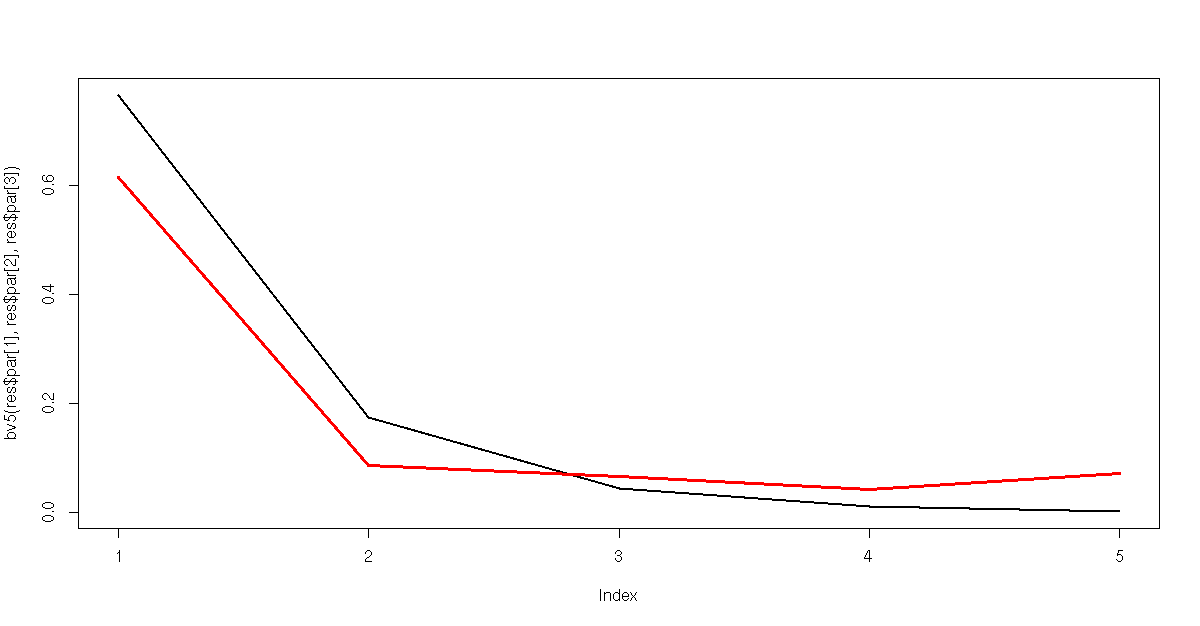
\includegraphics[scale=0.3]{fit_scaled_binomial_Q179.png}

This is quite imperfect but has some nice virtues: the parameters are  reasonable.  Unfortunately the optimiser is not sensitive enough to estimate the parameters without assistance.

\section{This Approach Will Work: Return to Understanding Process}

It's quite clear that this approach will yield good results after some work.  Now how can we demystify the locus of the biased coin flips?  Well, I would stretch out the process to two million years roughly in our evolutionary history.  

Let's say $n=200$ biased independent coin flips determine our conviction about some topic $T$, here we are looking at stealing.  We can distribute the coin flipping in two million years so that the recorded coin flips are in our genome for say 90\% or 80\% of the $n=200$ and leave the rest to actual brain and social development of individuals, including development of emotions, social understanding, and other psychological functions.  

\section{NLOpt Fit Full Vector}

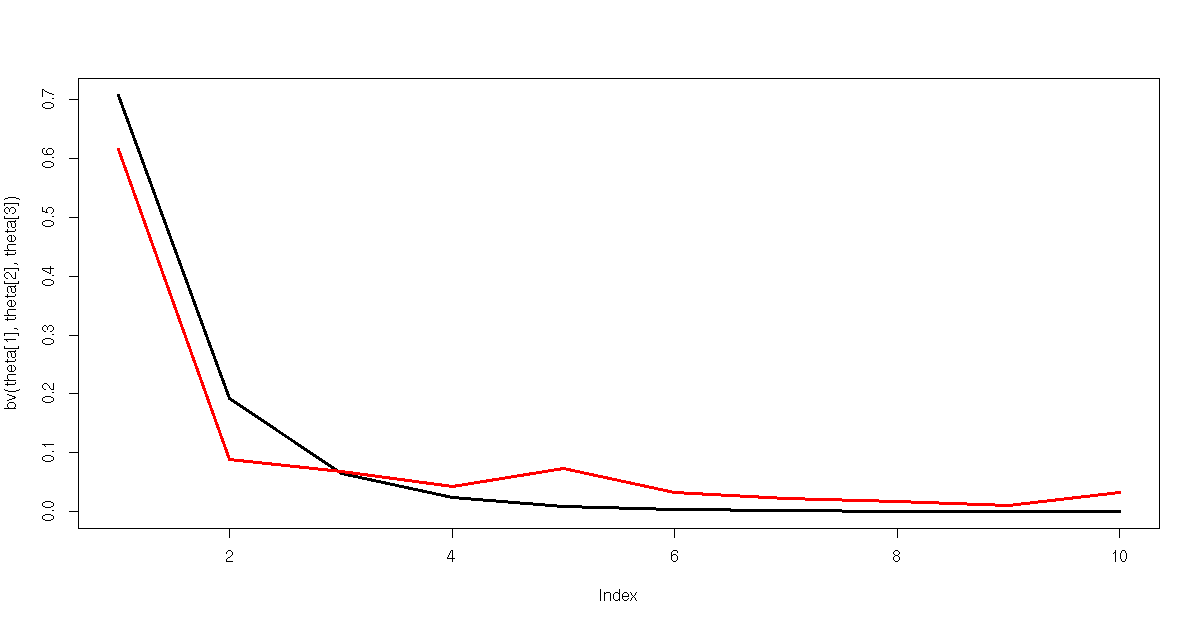
\includegraphics[angle=180,scale=-.3]{nlopt_fit_scaled_binomial_Q187.png}

\begin{verbatim}
lgchoose<-function(n,k){
  out<- log( n/(sqrt(2*pi)*k*(n-k))) + 
    n*log(n/exp(1)) - k*log(k/exp(1)) - (n-k)*log((n-k)/exp(1))
  out
}

binom<-function(p,n,k){
  exp(lgchoose(n,k)+k*log(p)+(n-k)*log(1-p))
}

bv<-function(p,n,alpha){
  z<-rep(0,10)
  for (k in 1:10){
    z[k] <- binom(p*alpha,n,k*alpha)
  }
  nrm(z) 
}

bv5<-function(p,n,alpha){
  z<-rep(0,5)
  for (k in 1:5){
    z[k] <- binom(p,n*alpha,k*alpha)
  }
  nrm(z) 
}


binom.err<-function( theta ){
  p <- theta[1]
  n <- theta[2]
  alpha <- theta[3]
  y <- bv5(p,n,alpha)
  print(y)
  norm( y - nrm(z[1:5]), type="2")
}

binom.err2<-function( theta ){
  p <- theta[1]
  n <- theta[2]
  alpha <- theta[3]
  y <- bv(p,n,alpha)
  #print(y)
  norm( y - nrm(z), type="2")
}
res<-nloptr(theta0,binom.err2,lb=lb0,
            opts=list("algorithm"="NLOPT_LN_NELDERMEAD",
                      "xtol_rel"=1.0e-6,
                      "maxeval"=5000,
                      "print_level"=1))

theta<-res$solution
plot(bv(theta[1],theta[2],theta[3]),type='l',lwd=3)
lines(as.numeric(y)[1:5], col='red',lwd=3)
> res

Call:

nloptr(x0 = theta0, eval_f = binom.err2, lb = lb0, opts = list(algorithm = "NLOPT_LN_NELDERMEAD", 
    xtol_rel = 1e-16, maxeval = 5000, print_level = 1))


Minimization using NLopt version 2.4.2 

NLopt solver status: 4 ( NLOPT_XTOL_REACHED: Optimization stopped because 
xtol_rel or xtol_abs (above) was reached. )

Number of Iterations....: 434 
Termination conditions:  xtol_rel: 1e-16	maxeval: 5000 
Number of inequality constraints:  0 
Number of equality constraints:    0 
Optimal value of objective function:  0.103779375754603 
Optimal value of controls: 1e-04 5 0.08003433

\end{verbatim}

\section{Scaled Binomial Log-Quadratic Model}

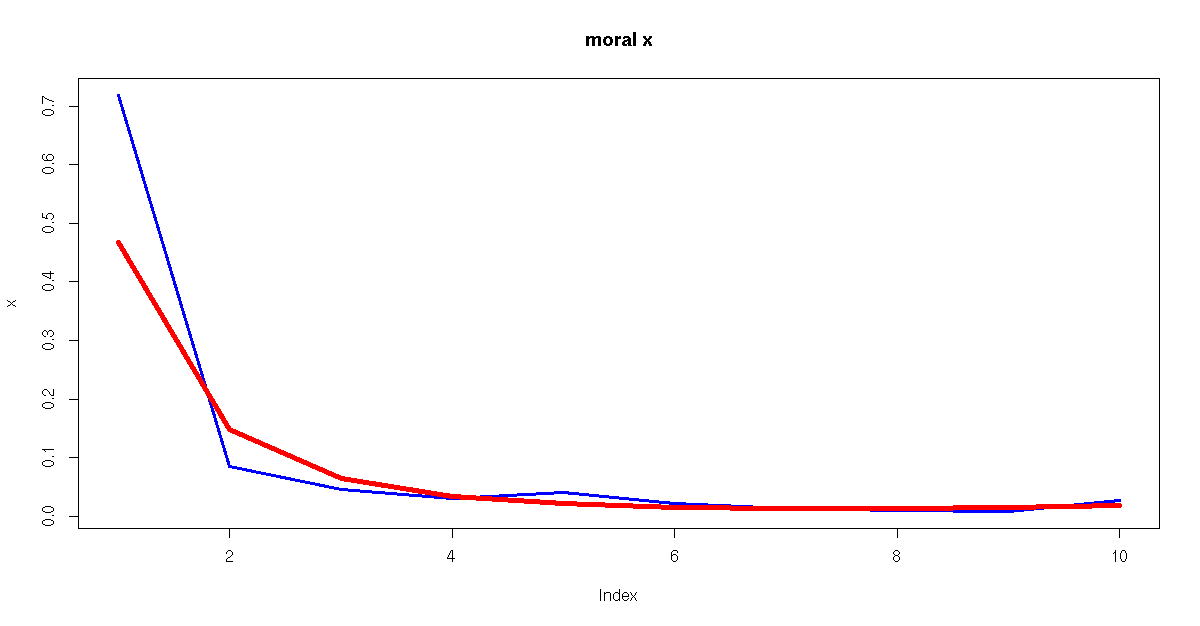
\includegraphics[scale=0.3]{fit_scaled_binom_log_quad.png}

\begin{verbatim}
lgchoose<-function(n,k){
  out<- log( n/(sqrt(2*pi)*k*(n-k))) + 
    n*log(n/exp(1)) - k*log(k/exp(1)) - (n-k)*log((n-k)/exp(1))
  out
}

binom<-function(p,n,k){
  exp(lgchoose(n,k)+k*log(p)+(n-k)*log(1-p))
}

bv<-function(p,n,alpha){
  z<-rep(0,10)
  for (k in 1:10){
    z[k] <- binom(p*alpha,n,k*alpha)
  }
  nrm(z) 
}

bv5<-function(p,n,alpha){
  z<-rep(0,5)
  for (k in 1:5){
    z[k] <- binom(p,n*alpha,k*alpha)
  }
  nrm(z) 
}


binom.err<-function( theta ){
  p <- theta[1]
  n <- theta[2]
  alpha <- theta[3]
  y <- bv5(p,n,alpha)
  print(y)
  norm( y - nrm(z[1:5]), type="2")
}

binom.err2<-function( theta, z){
  p <- theta[1]
  n <- theta[2]
  alpha <- theta[3]
  y <- bv(p,n,alpha)
  #print(y)
  norm( y - nrm(z), type="2")
}


fit.binom.quad<-function( z, theta0){

  f<-function(theta){
    binom.err2(theta,z)
  }

  res<-nloptr(theta0,f,lb=lb0,
              opts=list("algorithm"="NLOPT_LN_NELDERMEAD",
                      "xtol_rel"=1.0e-6,
                      "maxeval"=5000,
                      "print_level"=1))

  theta<-res$solution
  y<-bv( theta[1], theta[2], theta[3])
  
  qmod<-lm( log(z) ~ poly(log(y),2))
  print(summary(qmod))
  yp<-exp(predict(qmod))
  yp<-nrm(yp)
  yp
}

> 1- sum((y-x)^2)/sum(x^2)
[1] 0.8715459
\end{verbatim}

The R-squared of 0.87 is pretty good.

\section{Weighted Least Squares For Quadratic}

\begin{verbatim}

lgchoose<-function(n,k){
  out<- log( n/(sqrt(2*pi)*k*(n-k))) + 
    n*log(n/exp(1)) - k*log(k/exp(1)) - (n-k)*log((n-k)/exp(1))
  out
}

binom<-function(p,n,k){
  exp(lgchoose(n,k)+k*log(p)+(n-k)*log(1-p))
}

bv<-function(p,n,alpha){
  z<-rep(0,10)
  for (k in 1:10){
    z[k] <- binom(p*alpha,n,k*alpha)
  }
  nrm(z) 
}

bv5<-function(p,n,alpha){
  z<-rep(0,5)
  for (k in 1:5){
    z[k] <- binom(p,n*alpha,k*alpha)
  }
  nrm(z) 
}


binom.err<-function( theta ){
  p <- theta[1]
  n <- theta[2]
  alpha <- theta[3]
  y <- bv5(p,n,alpha)
  print(y)
  norm( y - nrm(z[1:5]), type="2")
}

binom.err2<-function( theta, z){
  p <- theta[1]
  n <- theta[2]
  alpha <- theta[3]
  y <- bv(p,n,alpha)
  #print(y)
  norm( y - nrm(z), type="2")
}


fit.binom.quad<-function( z, theta0){

  f<-function(theta){
    binom.err2(theta,z)
  }

  res<-nloptr(theta0,f,lb=lb0,
              opts=list("algorithm"="NLOPT_LN_NELDERMEAD",
                      "xtol_rel"=1.0e-6,
                      "maxeval"=5000,
                      "print_level"=1))

  theta<-res$solution
  y<-bv( theta[1], theta[2], theta[3])
  
  s<-1:10
  weights<-exp(-s/2)
  weights<-nrm(weights)
  qmod<-lm( log(z) ~ poly(log(y),2), weights=weights)
  print(summary(qmod))
  yp<-exp(predict(qmod))
  yp<-nrm(yp)
  yp
}
\end{verbatim}

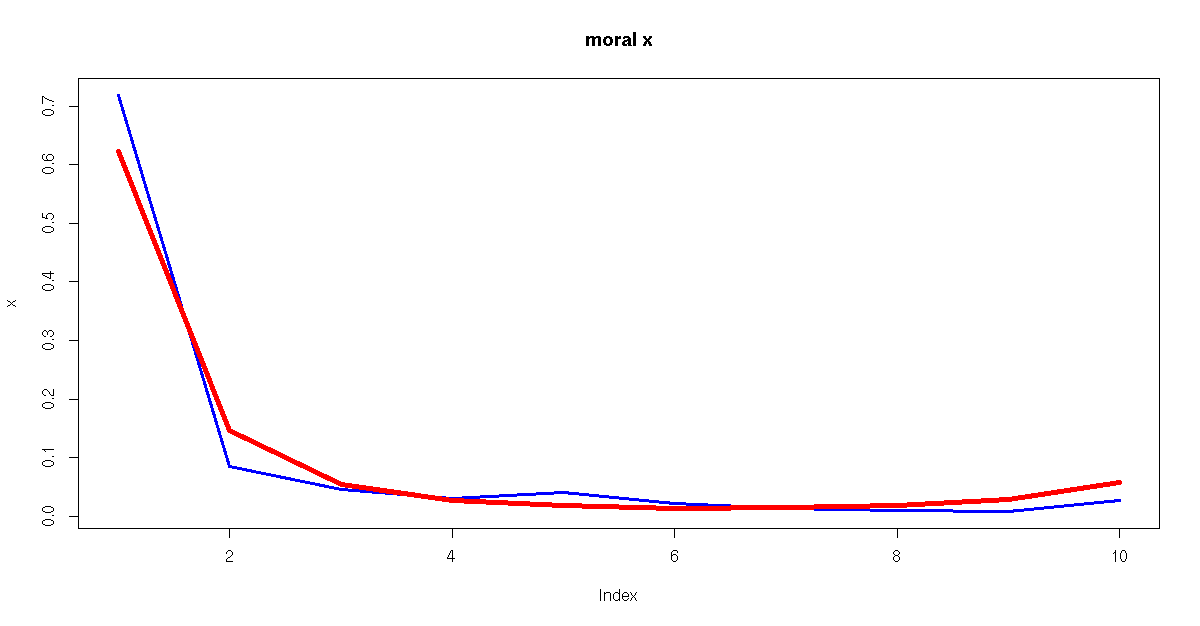
\includegraphics[scale=0.3]{wtls_log_quad.png}


\section{Flawless Test on New Data}

I tested on Q183, Prostitution. 

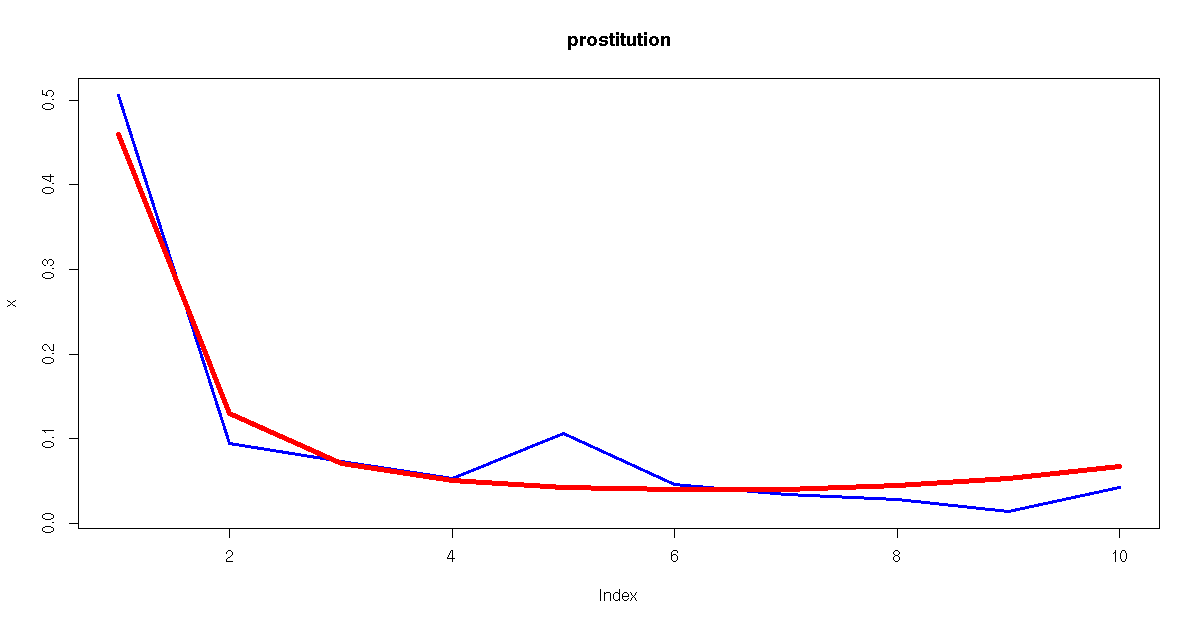
\includegraphics[scale=0.3]{fit_prost_may25.png}

Our R-squared was 0.967.  This is a great success!

\end{document}